\subsection{Custom Tags for JavaDoc}\label{sec:CustomTagsForJavaDoc}
The Javadoc\index{javadoc} tool allows to add custom tags that can be used within the documentation comments.

There are two different ways to add custom tags. The easier one is to configure them just on the command line for the tool, the more flexible one requires to write Java code that implements the \lstinline|jdk.javadoc.doclet.Taglet|\index{jdk.javadoc.doclet!Taglet} \autocite{ORACLE_DOC_TAGLET_INTERFACE} interface.

\subsubsection{Simple Custom Tags}\label{sec:SimpleCustomTags}
A simple custom tag is configured completely on the command line for the invocation of the Javadoc\index{javadoc} tool. This approach allows only block tag, but the text for these tags comes with full support for all inline tags.

\keeplisting{2}
The command line option for a new simple custom tag looks like this:
\begin{lstlisting}[numbers=none,language={}]
-tag <name>[:[<locations>]:<header>]
\end{lstlisting}

This specifies a custom block tag \texttt{<name>}. For the Javadoc\index{javadoc} tool to spell-check tag names, it is important to include a \texttt{-tag} option for every custom tag that is present in the source code, disabling (with \texttt{X} as the location) those that aren't being output in the current run.

\texttt{<locations>} is a combination of the letters below, in either uppercase or lowercase, that determine where the custom tag is allowed:
\begin{itemize}[nosep]
	\item{\texttt{A}: all declarations}
	\item{\texttt{C}: constructors\index{constructor}}
	\item{\texttt{F}: fields\index{field}}
	\item{\texttt{M}: methods\index{method}}
	\item{\texttt{O}: the overview page and other documentation files in doc-files subdirectories}
	\item{\texttt{P}: packages\index{package}}
	\item{\texttt{S}: modules\index{module}}
	\item{\texttt{T}: types (classes\index{class} and interfaces\index{interface})}
	\item{\texttt{X}: nowhere: the tag is disabled, and will be ignored, together with its argument}
\end{itemize}

Finally, \texttt{<header>} is the tag heading that is rendered in bold, followed by the tag's single argument in the next line.

\keeplisting{2}
For the command line option
\begin{lstlisting}[numbers=none,language={}]
-tag implNote:a:Implementation Note:
\end{lstlisting}
and the source code below
\keeplisting{10}
\begin{lstlisting}
/**
 *  {@summary Retrieves data from the queue.}
 *  
 *  @param  <T> The type of the data in the queue.
 *  @param  queue   The queue.
 *  @return An instance of
 *      {@link Optional}
 *      that holds the retrieved data.
 *  
 *  @implNote The method may not block; if the queue is (currently) empty,
 *      the implementation must return
 *      {@linkplain Optional#empty() empty}.
 */
public <T> T retrieveData( final Queue<T> queue );
\end{lstlisting}
the output will look like this:
\begin{center}
	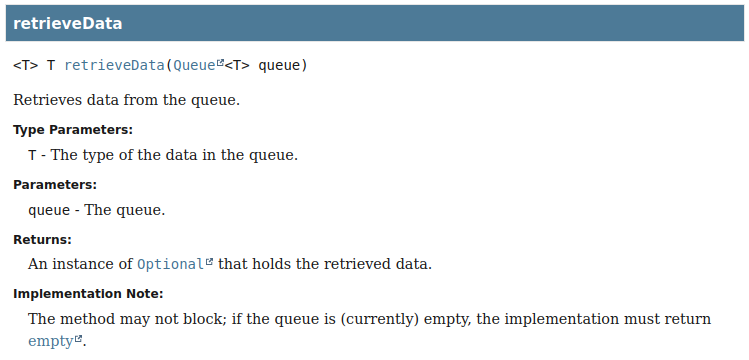
\includegraphics[scale=0.55]{comments/JavadocCustomTag1}
\end{center}

The colon (\bdq{:}) is always the separator. To include a colon in the tag name, escape it with a backslash. Omitting a value for \texttt{<header>} causes the name to be the heading, and if no location is specified, the tag can be used everywhere (same as \texttt{A} was specified). Refer also to \autocite{ORACLE_DOC_JAVADOC_MAN:StandardDocletOptions}.

The three tags below are defined per convention and widely used throughout the official documentation of the \Java API:

\paragraph{\lstinline|@apiNote|}\label{sec:TagApiNote}\index{apiNote@"@apiNote} Usage: \lstinline|@apiNote <text>|

This tag is used to provided some notes regarding the API.

\paragraph{\lstinline|@implNote|}\label{sec:TagImplNote}\index{implNote@"@implNote} Usage: \lstinline|@implNote <text>|

With this tag, you can add notes on how an implementation looks like (or should look like) to a program element.

\paragraph{\lstinline|@implSpec|}\label{sec:TagImplSpec}\index{implSpec@"@implSpec} Usage: \lstinline|@implSpec <text>|

This tag is added to provide information about the specification that is the base of the implementation for the respective program element.

\keeplisting{4}
To use these tags, they must be registered on the command line like this:
\begin{lstlisting}[numbers=none,language=sh]
javadoc -tag apiNote:a:API Note: \
        -tag implSpec:a:Implementation Requirements: \
        -tag implNote:a:Implementation Note:
\end{lstlisting}

%------------------------------------------------------------------------------

\subsubsection{Custom Taglets}\label{sec:CustomTaglets}
An introduction to implementing custom taglets would go beyond the scope of this book. However, the documentation for the \lstinline|jdk.javadoc.doclet.Taglet|\index{jdk.javadoc.doclet!Taglet} \autocite{ORACLE_DOC_TAGLET_INTERFACE} already provides a useful starting point.

Custom taglets do allow also the implementation of inline tags, on the other hand, they do not support to include the already existing inline tags.

If you want to use custom taglets, you have to provide the path to the implementing classes with the command line option \mbox{\texttt{-tagletpath}}; multiple locations are separated by a colon (\bdq{:}) on Linux/Unix operating systems, or by a semi-colon (\bdq{;}) on Windows.

Next each Taglet implementation class needs to be registered with the command line option \mbox{\texttt{-tagletclass}} (one entry per class).

I created a set of custom tags that I use regularly, and that I also recommend for your documentation comments. The respective library (\bdq{tquadrat’s Javadoc Extensions} or short \bsq{foundation-javadoc}) can be found at \autocite{TQUADRAT_ORG_FOUNDATION_JAVADOC}.

The command line for this would look like this:\footnote{Check the project's website at \autocite{TQUADRAT_ORG_FOUNDATION_JAVADOC} for the current version.}
\keeplisting{20}
\begin{lstlisting}
-tagletpath /path/to/org.tquadrat.foundation.javadoc-0.25.4.jar:\
/path/to/apiguardian-api-1.1.2.jar:/path/to/jakarta.activation-2.0.1.jar \
\
-taglet org.tquadrat.foundation.javadoc.AnchorTaglet \
-taglet org.tquadrat.foundation.javadoc.AuthorTaglet \
-taglet org.tquadrat.foundation.javadoc.FALSETaglet \
-taglet org.tquadrat.foundation.javadoc.HRefTaglet \
-taglet org.tquadrat.foundation.javadoc.IgnoreTaglet \
-taglet org.tquadrat.foundation.javadoc.ImageTaglet \
-taglet org.tquadrat.foundation.javadoc.IncludeTaglet \
-taglet org.tquadrat.foundation.javadoc.InspiredTaglet \
-taglet org.tquadrat.foundation.javadoc.ModifiedTaglet \
-taglet org.tquadrat.foundation.javadoc.NoteTaglet \
-taglet org.tquadrat.foundation.javadoc.NULLTaglet \
-taglet org.tquadrat.foundation.javadoc.ThanksTaglet \
-taglet org.tquadrat.foundation.javadoc.ToDoTaglet \
-taglet org.tquadrat.foundation.javadoc.TRUETaglet \
-taglet org.tquadrat.foundation.javadoc.UmlGraphLinkTaglet \
-taglet org.tquadrat.foundation.javadoc.UnderlineTaglet \
\
-tag hidden -tag note -tag param -tag return -tag throws -tag author -tag extauthor -tag thanks -tag modified -tag version -tag since -tag see -tag inspired -tag spec -tag provides -tag uses -tag UMLGraph.link -tag deprecated -tag todo \
-tag apiNote:a:API Note: \ 
-tag implSpec:a:Implementation Requirements: \
-tag implNote:a:Implementation Note: 
\end{lstlisting}

The purpose of the \texttt{-tag} options here is to determine the order in which the block tags appear in the final documentation. The command line for the Javadoc\index{javadoc} tool is further discussed in chapter \tqfullref{sec:RunJavadoc}.

\bdq{tquadrat’s Javadoc Extensions} provides the following custom taglets:

\keeplisting{4}
\paragraph{\lstinline|@anchor|}\label{sec:TagAnchor}  Usage: \lstinline|{@anchor #<anchor-name> <text>}|

This tag allows to add an HTML anchor to the generated documentation, where \texttt{\#<anchor-name>} is the name of the anchor to the given text. The hash symbol (\bsq{\#}) before the name of the anchor is mandatory!

%------------------------------------------------------------------------------

\keeplisting{5}
\paragraph{\lstinline|@author|}\label{sec:TagExtAuthor}  Usage: \lstinline|@author <name-text> - <email-address>| or \\
\lstinline|    @extauthor <name-text> - <email-address>|

This is a replacement for the \nameref{sec:TagAuthor}\index{author@"@author} tag that renders the given email address as a \texttt{mailto:} link in the generated documentation. It does not regard the option \mbox{\texttt{-author}} on the command line\footnote{This is valid for the current version 0.25.4 of the library; it may have changed for a later version.}.

The \lstinline|@extauthor| was introduced because some versions of the Javadoc\index{javadoc} did not allow to overwrite the standard \nameref{sec:TagAuthor}\index{author@"@author} tag.

%------------------------------------------------------------------------------

\paragraph{\lstinline|@false|}\label{sec:TagFALSE}  Usage: \lstinline|{@false}|

This is a shortcut for \lstinline|{@code false}|\index{code@"@code}.

%------------------------------------------------------------------------------

\paragraph{\lstinline|@href|}\label{sec:TagHref}  Usage: \lstinline|{@href <url> <text>}| or \lstinline|{@href <url>}|

With this tag, an HTML hyperlink can be added to the generated documentation; it will be placed inside the description text, but different from the \nameref{sec:TagLink} and \nameref{sec:TagLinkplain} tags, it allows to refer to arbitrary external resources, not only to other documented elements. Obviously, \texttt{<url>} is the target URL, while \texttt{<text>} is the clickable text. If the latter is omitted, the URL itself will be used instead.

%------------------------------------------------------------------------------

\paragraph{\lstinline|@ignore|}\label{sec:TagIgnore}  Usage: \lstinline|{@ignore <text>}|

With this tag text can be added to the documentation comment that is not shown in the generated documentation.

%------------------------------------------------------------------------------

\paragraph{\lstinline|@image|}\label{sec:TagImage}  Usage: \lstinline|{@image <url> <attributes>}|

The tag allows to add a picture to the generated documentation. \texttt{<url>} is the location of the image file, while \texttt{<attributes>} are HTML\index{HTML} attributes that are allowed for the \lstinline|<img>| tag.

%------------------------------------------------------------------------------

\paragraph{\lstinline|@include|}\label{sec:TagInclude}  Usage: \lstinline|{@include <source>:<process-mode>|

This tag allows you to include the contents of an external file in different ways, determined by the \texttt{<process-mode>}. It can be used to embed source code snippets into the documentation, but also to load text modules. 

\keeplisting{5}
Valid values for \texttt{<process-mode>} are:
\begin{itemize}[nosep]
	\item PLAIN
	\item ESCAPE
	\item MARKDOWN
	\item SOURCE
\end{itemize}

The code below includes the contents of the same file:
\keeplisting{8}
\begin{lstlisting}[language=Comment]
 …
 *  <hr>
 *  <p>{@include ${includes}/sample.html:PLAIN}</p>
 *  <hr>
 *  <p>{@include ${includes}/sample.html:ESCAPE}</p>
 *  <hr>
 *  <p>{@include ${includes}/sample.html:SOURCE}</p>
 *  <hr>
 …
\end{lstlisting}

For \bdq{\texttt{<process-mode> = PLAIN}} the output looks like this: 
\begin{center}
	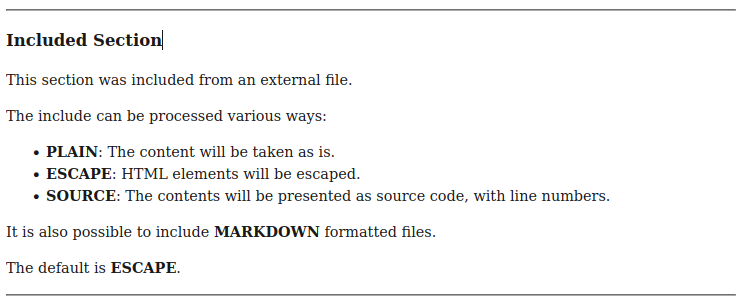
\includegraphics[scale=0.55]{comments/JavadocIncludePlain}
\end{center}
\bdq{\texttt{<process-mode> = ESCAPE}} is rendered like this: 
\begin{center}
	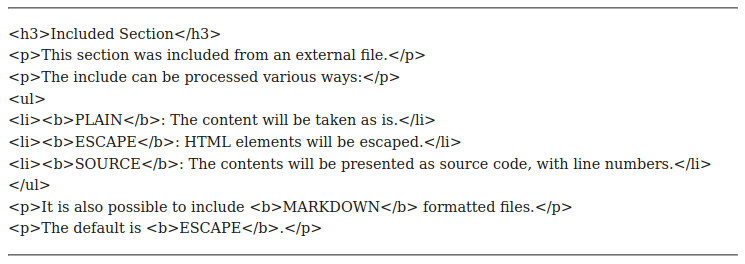
\includegraphics[scale=0.55]{comments/JavadocIncludeEscape}
\end{center}
And \bdq{\texttt{<process-mode> = SOURCE}} results a below: 
\begin{center}
	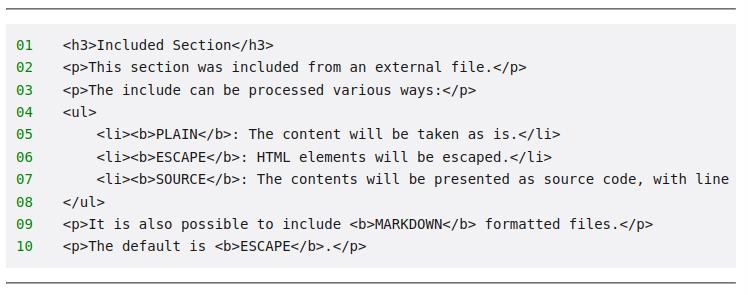
\includegraphics[scale=0.55]{comments/JavadocIncludeSource}
\end{center}

For more details on the \bdq{\{\nameref{sec:TagInclude}\}} tag, refer to \autocite{TQUADRAT_ORG_FOUNDATION_JAVADOC}.

%------------------------------------------------------------------------------

\paragraph{\lstinline|@inspired|}\label{sec:TagInspired}  Usage: \lstinline|@inspired <text>|

Sometimes a piece of code was inspired by a document of some kind, a description of an algorithm, a product white paper, or whatever. This tag allows you to add a reference to that source of inspiration.

Refer also to \nameref{sec:TagSpec}\index{spec@"@spec}, \nameref{sec:TagImplNote}\index{implNote@"@implNote}, \nameref{sec:TagImplSpec}\index{implSpec@"@implSpec} and \nameref{sec:TagApiNote}\index{apiNote@"@apiNote} as they are somehow related. In particular if the reference to the inspiration is only a URL, the \nameref{sec:TagSpec}\index{spec@"@spec} is preferred.

%------------------------------------------------------------------------------

\paragraph{\lstinline|@modified|}\label{sec:TagModified}  Usage: \lstinline|@modified <name-text> - <email-address>|

This is a variant of the \nameref{sec:TagExtAuthor} tag. It is meant to provide the name of the developer that modified the respective element without claiming to be an author.

%------------------------------------------------------------------------------

\paragraph{\lstinline|@note|}\label{sec:TagNote}  Usage: \lstinline|@note <text>|

With this tag, it is easy to add important notes to the generated documentation for an element. All notes will be added to a bullet list placed immediately beneath the documentation text. The text for the \lstinline|@note| tag is somehow limited as it does not allow other Javadoc tags.

%------------------------------------------------------------------------------

\paragraph{\lstinline|@null|}\label{sec:TagNULL}  Usage: \lstinline|{@null}|

This is a shortcut for \lstinline|{@code null}|\index{code@"@code}.

%------------------------------------------------------------------------------

\paragraph{\lstinline|@thanks|}\label{sec:TagThanks}  Usage: \lstinline|@thanks <name-text> - <email-address>|

Use this tag to mention someone who provided input to the respective element without being an author; that person might have wrote an article about the algorithm that was implemented by this element, or they may have reported a bug.

Same as for the \nameref{sec:TagExtAuthor} and the \nameref{sec:TagModified} tags, the email address will be rendered to a \verb#mailto:# link in the generated documentation.

%------------------------------------------------------------------------------

\paragraph{\lstinline|@todo|}\label{sec:TagTodo}  Usage: \lstinline|@todo <todo.md>|

This tag copies the contents of the Markdown\index{Markdown} file specified by \texttt{<todo.md>} into the generated documentation. This is meant as a ToDo list or list of open issues, and that is reflected by the heading that is added to the generated documentation.

%------------------------------------------------------------------------------

\paragraph{\lstinline|@true|}\label{sec:TagTRUE}  Usage: \lstinline|{@true}|

This is a shortcut for \lstinline|{@code true}|\index{code@"@code}.

%------------------------------------------------------------------------------

\paragraph{\lstinline|@UMLGraph.link|}\label{sec:TagUMLGraph}  Usage: \lstinline|@UMLGraph.link|

This adds an UML graph for the current class to the generated documentation.

%------------------------------------------------------------------------------

\paragraph{\lstinline|@underline|}\label{sec:TagUnderline}  Usage: \lstinline|{@underline <text>}|

Use this tag to add underlined text to the generated documentation.

%==============================================================================
% End of file!!
%==============================================================================

